%************************************************
\chapter{Project Information}
\label{chp:Project Information}
%************************************************
This practicum is primarily an exploration into FreeBSD kernel modules with respect to covert data communications. The main functionality of this system will be to allow any single node within the network to exfiltrate data from any other node within the network. However, with respect to being a covert network, the kernel module will be responsible for misreporting the state of network connections to the operating system. This will make any cursory inspection of active network connections mislead the operator into thinking everything is operating normally.

In addition to data exfiltration from any particular node in the network, one will also be able to make use of the network as a proxy for standard HTTP requests; much like a Tor\footnote[1]{\url{https://www.torproject.org}} network.

Throughout my exploration of this practicum, I will attempt to implement the following major features:
\begin{itemize}
	\item Network topology modelled after mesh networks\footnote[2]{\url{http://en.wikipedia.org/wiki/Mesh_networking}}.
	\item Kernel-based encryption for all network communication.
	\item Ability to use the network in a Tor-like fashion for standard HTTP requests.
	\item Exfiltration of data from any node within the network.
	\item Near real-time interaction with any node via standard command-line interface.
	\item Implementation of client/server functionality as loadable FreeBSD kernel modules.
	\item Kernel modules mask their existence from any users on the system.
	\item Kernel modules hook into system network calls in order to hide traffic from internal inspection within the system.
\end{itemize}

\section{Background Information}
For a network to be as robust as possible, topology matters. In this case, I have chosen a standard mesh topology where each node can connect to any other node within the network. However, this doesn't necessarily mean that each node is constantly connected to every other node in the network at once. In fact, it will be how packets are routed from node to node that will adopt a mesh-like topology.

\begin{figure}[h!]
	\centering
	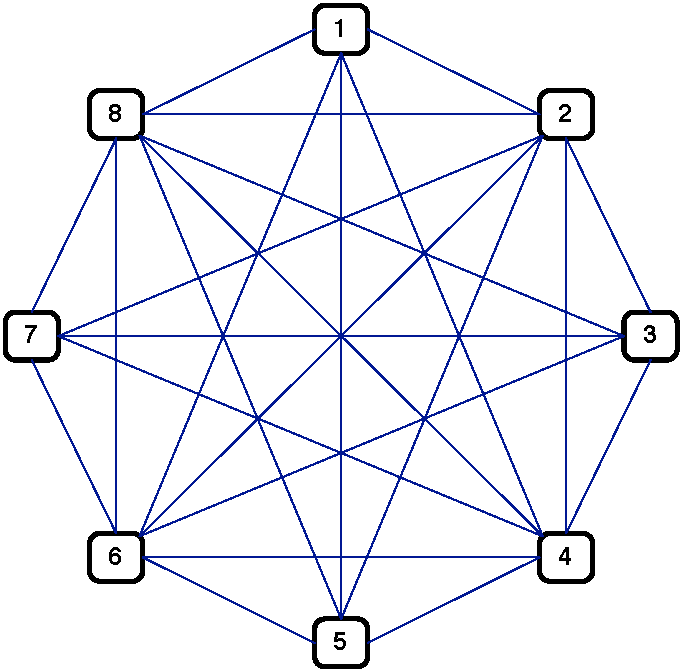
\includegraphics[width=1.0\textwidth]{MeshNetwork}
	\caption{Possible connections within a mesh network.}
\end{figure}

From the above graph, once and see that the network consists of nodes where each node is connected to every other node in the network. This is a basic mesh network topology. Such a network is very resilient to any type of disruption, for the removal of any nodes will not disrupt the network as a whole. From a security standpoint, if any particular node were compromised (by the good guys in this case), one could ascertain the identity of all member nodes within the network. However, this does not necessarily mean that the identity of the individual who compromised the network is specifically at risk -- more on this later.

Routing within the network will depend on which node the infiltrator is connected to. For example, if the infiltrator is communicating with node \#1, but wants to exfiltrate data from node \#8 or make a Tor-like HTTP request, the system will route the request along a random path using a random number of hops\footnote[3]{The hops may take the form of rand($1...n-1$) nodes.}. Communication with node \#1 (in order to reduce the chances of discovery) will be accomplished with specially formatted ICMP messages with a forged source address.

\begin{figure}[h!]
	\centering
	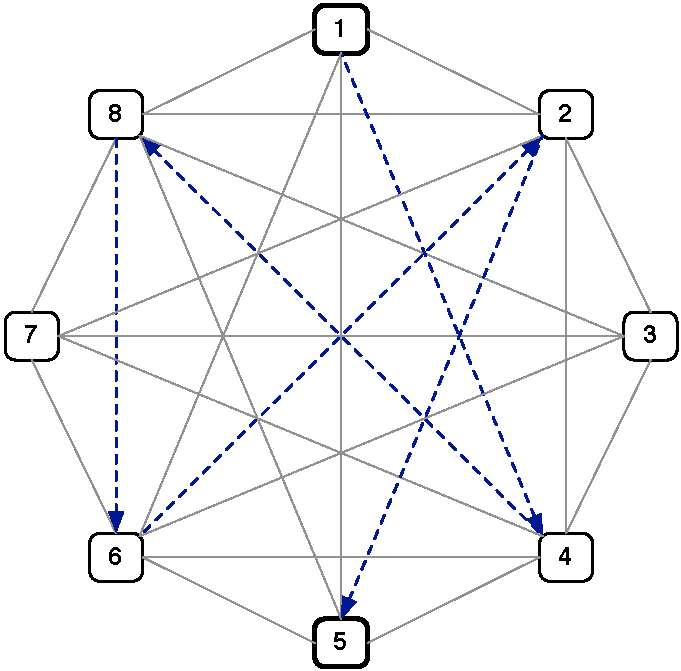
\includegraphics[width=1.0\textwidth]{MeshRouting}
	\caption{Example of random routing from node \#1 to node \#8.}
\end{figure}

In order to reduce the chances of the infiltrator's identity being discovered, we need to implement a way for the client/server application to be hidden from casual inspection of the system itself. This can be achieved though implementing the client/server software as a loadable kernel module. As explained in \emph{Fun and Games with FreeBSD Kernel Modules}\footnote[4]{\url{http://www.r4k.net/mod/fbsdfun.html}}, with a kernel module we can both hide the process itself (along with the kernel module we loaded and any subsequent children created) and even the desired network activity from the rest of the system completely. What this would mean is that if the user were to preform a `ps -aux' or a `netstat -nav' command, neither�s results would betray the existence of the kernel module itself. Additionally, network traffic itself may possibly be hidden from the view of a raw packet dump using `tcpdump'\footnote[5]{This may possibly need to be compiled into the kernel, as this falls outside the domain of simply hooking into system calls.}.

\clearpage
\section{Methodology}
The exploration of this practicum can be divided up into several discrete modules, which can then be integrated. The following sections will briefly outline each module and its function.

\subsection{Network Building}
Given a list of node from which to build a network, the initial node will communicate the entire list of addresses with a random node in the network. As stated earlier, all communications between nodes will be encrypted. This node will then communicate the entire list of addresses with another random node. The difference here is that as we progress through the mesh, nodes to which the list has already been communicated will be marked in order to avoid randomly connecting with a node that has already received the list of addresses.

What this means is that the number of possible random connections will decrease until there is only one possible node to which the list of addresses can be communicated.

In the event that a node is removed from the network or becomes inaccessible, that node will be removed from each node's list of possible connections. However, if the offending node becomes active once again, it will be reincorporated into the network as soon as it initiated communication with any of the active nodes.

\subsection{FreeBSD Kernel Modules}
One of the main features of this project is the creation of a loadable kernel module for FreeBSD that is able to mask its presence from the process table and selectively hide network traffic from utilities such as tcpdump. In order to achieve this, the kernel module needs to intercept the various ways information about processes is obtained. Also it will have to keep track of which processes need to be hidden. Every process is recorded in a struct proc. By extension, hiding network connections also requires intercepting system calls.

\subsection{Data Transfer}
With the kernel module hiding the associated network traffic from the user, we may be able to forgo data obfuscation within TCP/IP headers, thereby allowing for higher throughput while still remaining unnoticed to the user. As such, large transfers of data may be able to go unhindered. However, if this is not the case (after further experimental research into FreeBSD kernel modules), implementation of an obfuscation scheme may become necessary.

\subsection{Encryption}
With normal user-land software, network communication can be easily encrypted using OpenSSL libraries. However, because kernel modules do not have access to anything that is not provided within the kernel itself, I will need to make use of any built-in encryption that the kernel provides. Failing this, I will need to implement my own encryption routines from scratch. 

Given this limitation, key exchange between nodes could be simplified by using a single encryption key across the entire network. It may be possible to devise a scheme where each node's connection with another uses a different key, but this entirely hinges on the type of encryption the kernel provides, if any.

\subsection{Testing \& Implementation Environment}
Ideally, only a single virtualized copy of FreeBSD using FreeBSD will be needed. In order to simulate a multitude of individual systems with a single virtualized copy of FreeBSD, a feature of FreeBSD called �jails� may be employed. With FreeBSD jails it is possible to create various different virtual machines, each of them having their own set of utilities installed and their own configuration. This makes it a safe way to try out software. For example it is possible to run different versions or try different configurations of Apache in different jails. And since the jail is limited to a narrow scope, the effects of a misconfiguration or mistake (even if done by the in-jail superuser) does not jeopardize the rest of the system's integrity.

However, the use of loadable kernel modules from within a jail may be suspect. If it is not possible to use FreeBSD jails along with kernel modules, a virtualization environment using VMWare where each node has its own virtualized copy of FreeBSD could be implemented. This would allow for the concurrent running of multiple iterations of FreeBSD in order to test a network of nodes. The memory requirements of a base FreeBSD system are minimal, therefore with 21 (for example) virtualized environments, each with 256MB of RAM, only a total of 5376MB of RAM will be required. The current testing system has 8192MB of RAM and makes use of a high-end Intel Core i7 processor. If this proves to be too much for the system, virtualization may be spread among several computer systems.

\subsection{Prototyping}
Given the exploratory nature of this practicum, I will be going with an incremental software prototyping approach to development. Small-scale mock-ups of each part of the system, outlined above, will be developed following an iterative modification process until the prototype evolves to meet the system�s requirements.

For instance, the first task will be that of creating a loadable FreeBSD kernel module that is able to mask specific network connections. This will then expand into having the kernel module intercept and manage communications between multiple nodes. However, because of the exploratory nature of this practicum, a rigid development and integration plan is not feasible. This is why I will be focusing on creating iterative prototypes, slowly adding features to each iteration until a base level of functionality has been achieved.

\clearpage
\section{Technologies Used}

There is a prolific amount of information on the Internet with respect to using kernel modules in order to `root' or exploit Linux or Windows systems. However, such information with respect to FreeBSD systems is either exceptionally out of date (and therefore no longer applicable or relevant) or simply non-existent. Because of this limiting factor, my explorations into accomplishing the goals of this project will have little or no precedent.

\noindent
\textbf{Programming Language:} C/C++ \\ \\
\textbf{Operating System:} FreeBSD 9.0 \\ \\
\textbf{Network Topology:} Mesh Network \\ \\
\textbf{Security Implementation:} Process and network connection hiding using FreeBSD loadable kernel modules. Direct interception of system calls in order to sanitize undesirable connection information from any user on the system. \\ \\
\textbf{Virtualization Environment(s):} FreeBSD running as a guest on VMWare workstation 8.0. Additionally, the virtualized FreeBSD environment may make use of jails in order to virtualize and simulate any size of network. For example, I may initiate 32 jail environments in order to simulate a mesh network of 32 nodes. Each virtualized environment will be able to collect data particular to that environment, such as raw TCP/IP dumps and process information.

\clearpage
\section{Testing Plan}
Much of this project's work lies within loadable FreeBSD kernel modules. Unfortunately, unlike user-land applications, there exists no established procedure for testing, such as unit testing. However, this does not mean that a testing procedure cannot be established for kernel modules.

\subsection{Kernel Module Testing}
In order to test a kernel module, the module needs to output to a standard character device (for example /dev/charout). This is analogous to a developer adding printf("It works!") to somewhere within a standard program. Obviously this is not an ideal situation, but given the nature of kernel modules, one cannot implement established testing procedures such as unit tests.

Whenever the kernel module successfully intercept a system call, this fact can be written out to a standard character device. Similarly, communication with other nodes in the network can be output to a character device as well.

Essentially, all testing with regards to the kernel module will have to be done via print messages output to a character device. Because this is an exploratory project, I cannot be more definite as to testing procedure in this regard.

\subsection{Unit Testing outside of the Kernel Module}
I will be making use of a unit testing framework for C called Check\footnote[5]{\url{http://check.sourceforge.net/doc/check_html/index.html}}. It was inspired by similar frameworks that currently exist for most programming languages; the most famous example being JUnit for Java. The incremental test and code approach will provide three main benefits:

\begin{enumerate}
	\item Because the unit tests use the interface to the unit being tested, they allow the developer to think about how the interface should be designed for usage early in the coding process.
	\item They help the developer think early about aberrant cases, and code accordingly.
	\item By providing a documented level of correctness, they allow the developer to refactor.
\end{enumerate}

As noted, unit testing cannot be used with loadable kernel modules. As such, any unit testing that does occur will be limited to any software created that lies outside of the kernel. For instance, a helper daemon will be required to facilitate interpretation of command-line interface-type commands. That is whenever a command to execute something on the command-line (such as rm -rf somefile), the kernel module will need to pass that information to a character device which is read by the daemon and then executed.

Given the nature of unit testing, the process will involve the creation of functional code and then the creation of tests to validate said code�s sanity. This will inevitable lengthen the amount of time spent coding, but it will inevitable lead to fewer issues as we near completion.

\subsection{Functional Testing}
Unit testing can only go so far when it comes to the fully functional result. With the code fully tested, the actual functionality of the system will need to be tested. In order to achieve this, functional testing will be split into the following major activities:

\begin{itemize}
	\item \textbf{Network Structure} - Validate that each node is connecting with the appropriate nodes within the mesh. This will be verified by disabling any and all network connection hiding mechanisms of the system and using the tool tcpdump to verify that each node is only talking to the node it should be.
	\item \textbf{Kernel Module: Process Hiding} - Validate that the any associated processes and loaded kernel modules do not show up in the process table. Additionally, examine whether signs of the application can be traced using FreeBSD�s dtrace utility.
	\item \textbf{Kernel Module: Network Connection Hiding} - Validate that associated network connections do not show up when using `netstat -nav' and that network traffic cannot be seen when using tcpdump.
	\item \textbf{Kernel Modules: Loading \& Unloading} - Validate that the system responds appropriately to loading and unloading the kernel module. Forced unloading of the module should be intercepted and disabled by the kernel module itself and loading unassociated modules should be permitted while the custom kernel module is running.
	\item \textbf{Encryption \& Decryption} - Data encryption can be verified by having the kernel module output example encrypted and unencrypted data to a character device.
\end{itemize}

\clearpage
\section{Schedule Estimates}
\textbf{Total Schedule Budget:} $\sim$435 Hours

\subsection{Research}
$\sim$60 Hours

A great deal of exploratory research into FreeBSD kernel modules will need to be accomplished before any real programming in earnest can be accomplished. Specific research into process hiding and network connection hiding requires a lower level understanding of the FreeBSD kernel and its system calls.

Additionally, research into appropriate encryption technologies as well as the limitations of using a FreeBSD jails setup with respect to loadable kernel module support will also need to be looked into.

\subsection{Environment Setup}
$\sim$10 Hours

Installation and configuration of a virtualized FreeBSD environment using VMWare for programming and testing along with the associated FreeBSD jailed environments for full scale testing.

\subsection{Proof of Concept Prototypes}
$\sim$80 Hours

Development of a proof of concept prototype loadable kernel module for FreeBSD that accomplishes a simplified version of the goals required for the final kernel module. Failure to create an adequate prototype at this stage will require a changing to a data obfuscation scheme using TCP/IP headers instead of making the traffic at the kernel level. Success of this proof of concept is imperative to the project as a whole.

\subsection{Programming}
$\sim$210 Hours

Development in earnest, including unit tests for each module of code produced. This also included final integration of the code. The high budget time for this section is to take into account the uncertainty involved in developing in the kernel space for a system that is relatively little used.

\subsection{Testing \& Debugging}
$\sim$50 Hours

Final testing and debugging, which is inevitable. In addition to troubleshooting any problems that made it this far into the development cycle, testing will begin to produce documented results for use in the final report. All data produced throughout this phase of the project should be documented and saved.

\subsection{Documentation \& Final Report}
$\sim$25 Hours

Collation of all the testing documentation and construction of the final report along with all supporting data and analysis.
